\chapter{Related Work}
This chapter presents the related work on which this project was built on. The basis was the work done at General Acoustics e.K. particularly from Dipl.-Ing. (FH) Jan Schirrmacher in previous projects containing an ADCP. Afterwards an in-depth introduction on the used ADCP from Rowe Technologies, Inc.\cite{rowe} will provide the needed background information in this field. Finally, the used external libraries will be presented to give background information needed further in the report.

\section{General Acoustics e.K.}
Due to previous projects with ADCP's a lot of knowledge about the technology was already available from General Acoustics e.K. A look at the algorithms of the current ADCP parser as well as other libraries used in this context gave a good introduction into the problem and helped a lot in architectural decisions. The libraries were developed by Jan Schirrmacher in Delphi and, thus, only available for Windows. Listing 2.1 shows a code snippet in Delphi from the ADCP parser function currently used in various applications. In the snippet are two steps of the parser presented, in \texttt{psStartSequence} the parser tries to find a binary sequence in the incoming binary data. After the sequence is found the parser reads a header in \texttt{psHeader} from the data stream. Without help like the code in Listing 2.1 the implementation would probably not have been possible in the time-frame of this project.

One application developed by Jan Schirrmacher that contained the parser code from Listing 2.1 was the so called \texttt{BurstReporter}. It parses ADCP data and presents them in a human readable text file. This tool was heavily used to verify the correctness of the software developed in this software project.
\vspace{5em}
%delphicode 
\begin{lstlisting}[language=Delphi, caption=Exemplary ADCP parser code from Jan Schirrmacher]
function TParser.Scan :boolean;
...
begin
  FEOF := false;
  result := false;
  try
    case FStep of
    psStartSequence:
      begin
        FEnsembleComplete := false;
        if FQueue.Find(TEnsemble.STARTSEQUENCEbyte, sizeof(TEnsemble.STARTSEQUENCEbyte), Index) then begin
          // Position im Host-Stream rekonstruieren, damit Dateiposition sich gemerkt werden kann
          FEnsemblePosition := FQueue.HostPosition - FQueue.Available + Index;
          FQueue.Drop(Index + sizeof(TEnsemble.STARTSEQUENCEbyte));
          FStep := psHeader;
          if Index>0 then
            MsgOut(Format(SErrSyncFailedFmt, [Index]), false);
        end else begin
          FEOF := true;
          if FQueue.Available=FQueue.Capacity then begin
            MsgOut(Format(SErrSyncFailedFmt, [FQueue.Available]), false);
          end;
        end;
      end;
    psHeader:
      begin
        // Header lesen
        if Read(FEnsemble.Header, sizeof(FEnsemble.Header)) then begin
          if FEnsemble.Header.EnsembleNumber<>not FEnsemble.Header.InvEnsembleNumber then
            MsgOut(SErrInvalidHeader)
          else if FEnsemble.Header.PayloadSize<>not FEnsemble.Header.InvPayloadSize then
            MsgOut(SErrInvalidHeader)
          else begin
            SetLength(FEnsemble.Payload, FEnsemble.Header.PayloadSize);
            FStep := psPayload;
          end;
        end else
          FEOF := true;
      end;
...
\end{lstlisting}
\vspace{4em}
\section{Acoustic Doppler Current Profiler}
An Acoustic Doppler Current Profiler (ADCP) is a hydro-acoustic instrument or sonar device that is used to measure water velocities in separated layers over a certain range that is defined by the acoustic frequency. Essentially, the ADCP emits a sound signal of a specific frequency and measures the return frequency that is received from backscatter via particles in the water column \cite{adcp_def}.

The reference ADCP used for this project is produced by Rowe Technologies Inc. \cite{rowe}. It has four horizontal pistons and one vertical piston, also known as beams. Beams emit the waves used to measure the flow currents and directions. The beams of the ADCP can be seen in Figure 2.1 represented as red circles. In the figure, the ADCP is mounted on a self-designed structure to stand stable and well-positioned on the ocean floor.

\begin{figure}[h]
\centering
      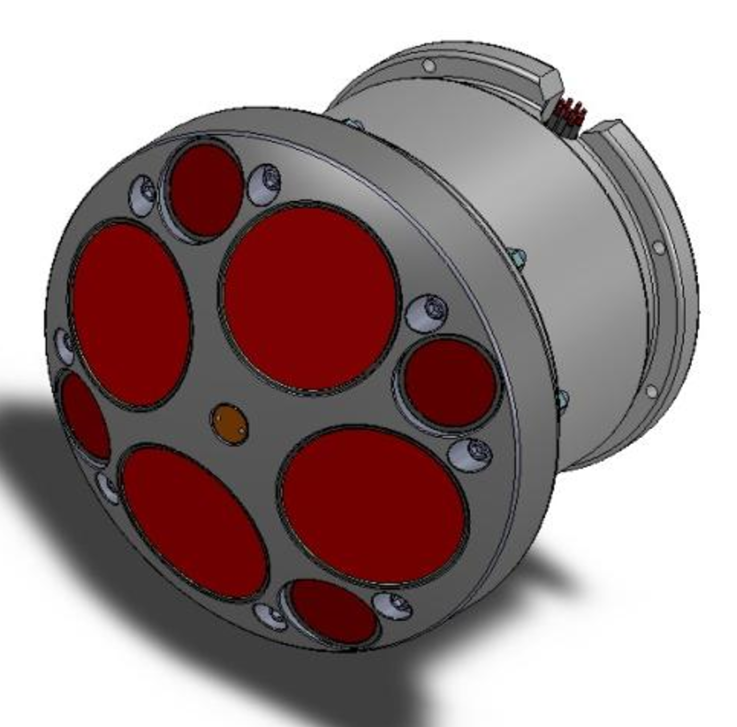
\includegraphics[width=0.6\textwidth]{adcp}
        \caption{A picture of the ADCP referenced in this project.}
\end{figure}

The used ADCP (Figure 2.1) is configured to measure a maximum of 15-meter distance divided into 30 separate layers, also called bins, of 0.5 m height. The four horizontal beams are used to measure the flow currents and directions, internal signal processing is used to calculate the correct local Cartesian coordinates (East, North, Up) based on the ADCP position and heading, pitch, and roll angles. The single beam is used to measure the water level.\\
The ADCP is configured to ping at 6Hz always alternating either a horizontal or a vertical ping. It operates in bursts, one burst every 10 minutes. One burst consists of 2048 pings where 1024 are horizontal and 1024 are vertical pings. A ping is also called ensemble therefore, a burst is defined as a collection of 2048 ensembles, measured over a period of ~6-7 minutes. An ensemble contains the data of one ping, the structure of the data is presented further-on in Section 2.2 of the report. The collected data is then sent burst-wise over RS-485 at 460800 Bd\footnote{\label{foot:2} Bd (Baud) is the unit for the symbol rate or modulation rate in $[T^{-1}]$, in general symbols per second.} to a data-logger on the offshore platform.

An ADCP ensemble consists of three sections. The first section is a 32 Byte header. The header consists of 16 Byte containing 0x80, followed by a four byte \texttt{uint32} ensemble number. The next four bytes contain the ones-compliment of the ensemble number. The last eight bytes contain the \texttt{uint32} payload size in bytes as well as its ones-compliment.\\
The middle section contains the payload as MATLAB v.4 \cite{matlab} file. A MATLAB-file may contain one or more matrices. The matrices are written sequentially to a file, forming a continuous byte stream. Each matrix starts with a fixed-length 20 Byte header that contains information describing certain attributes of the matrix. The header consists of five long four byte integers. After the header the matrix data follows in the numerical format specified in the header. The data contains rows $\times$ columns number of elements.
The payload of an ensemble contains a series of matrices named E000001 to E000015. Depending on the ensemble type not all matrices may be available.\\
The last section is a four byte Cyclic Redundancy Check (CRC) checksum over all bytes in the payload. The first two bytes are always 0, the second two bytes contain the CRC16 value. The value is based on the International Telegraph and Telephone Consultative Committee (CCITT) 16 Bit algorithm following the formula 

$$ x^{16} + x^{12} + x^5 +1$$

with CRC seed\footnote{\label{foot:3} The CRC seed is the value used to initialize the initial checksum or CRC register before the computation of the CRC.} of value 0.

If the 32 Byte header is removed from each ensemble, MATLAB is able to read in the ensembles.
\begin{figure}[h]
\centering
      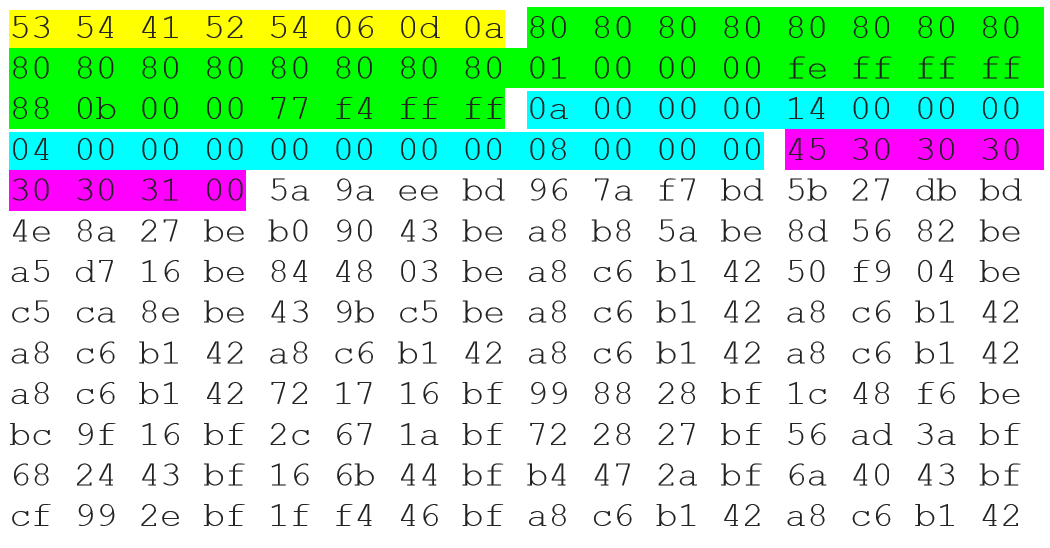
\includegraphics[width=0.7\textwidth]{hexdump}
        \caption{A hex-capture of the first few bytes from an ensemble.}
\end{figure}
Figure 2.2 shows the first few bytes of an ensemble.
\begin{itemize}
\item Yellow marked is the word \texttt{START} followed by 0x14 0x10 (carriage return line feet also called \texttt{CRLF}). This was captured when the ADCP was started.
\item Green colored is the 32 Byte ensemble header, it begins with the 16 Byte of 0x80.
\item Cyan is the MATLAB v.4 matrix header containing four integer values which are set to 10, 20, 4, and 8.  
\begin{itemize}
\item The 10 indicates the matrix contains 4 Byte floating point numbers. 
\item 20 is the number of rows in the matrix which is the number bins in the ADCP profile. 
\item 4 is the number of columns which is the number of ADCP profile beams.  
\item 8 is the number of bytes in the matrix name.  
\end{itemize}
\item Pink is the matrix name ``E000001''.
\item Following that there are $4 \times 20 = 80$  floating point numbers in the matrix (not all shown in Figure 2.2 due to the size of the ensemble).
\item The next matrix ``E000002'' starts after the last floating point number... and so on until all of the matrices in the ensemble are read in.
\item The end of the ensemble has 4 more bytes that are used as a checksum. 
\item The next ensemble starts with a 32 Byte header just like the previous one and contains the same matrix names repeated but with new data. 
\end{itemize}

To present the content of all 15 matrices would go beyond the scope of this report and, thus, only the important matrices are described. The other matrices contain additional information e.g. ping quality, and are thrown away in the parsing process of the developed software to reduce the size of the logged files. In Appendix A the official documentation of all matrices was attached.\\
The matrices that are used for further processing from General Acoustics e.K., e.g. for wave analysis, are:
\begin{itemize}
\item ``E000001'' - Bins $\times$ beams of single precision floating points containing the beam coordinate velocity profile data as measured along each beam. The data is useful for diagnostic purposes and for when the user wants to perform their own transformation. In the context of this project the data is only used for further wave analysis, and only from the vertical pings.
\item``E000003'' - Bins $\times$ beams of single precision floating points containing the earth coordinate velocity profile in m/s. 
\item ``E000008'' - Twenty-two 32 Bit integers containing various ensemble data, the ensemble number, time-stamp, number of bins and beams as well as the ADCP system configuration.
\item ``E000009'' - Thirteen single precision floating points containing various ancillary data, e.g. water pressure and water temperature.
\item ``E000015'' - 1 + 3 $\times$ beams of single precision floating points containing e.g. the water level. 
\end{itemize}

\section{Libraries}
For the implementation of this project, a number of external libraries were used to simplify the development process. The decision for or against various libraries is justified in Chapter 3, at this point, only the libraries used in the implementation are described.
\subsection{Boost C++ Libraries}
Boost \cite{boost} is a collection of libraries for the C++ programming language. It contains over eighty individual and portable libraries to support a wide range of use cases. The libraries are licensed under Boost Software License \cite{boostliz}, which are designed to be used for both free and proprietary software. A lot of Boost libraries get accepted for new C++ standards, the latest big incorporation was when the C++11 standard was introduced \cite{booststd}. Most Boost libraries are header only, consisting only in-line functionality and templates, some other libraries have to be compiled separately before they can be used.

In the development of this software project, mainly the following boost libraries were used:
\begin{itemize}
\item \texttt{boost::asio} - Boost.Asio is a cross-platform C++ library for network and low-level I/O programming that provides developers with a consistent asynchronous model using a modern C++ approach \cite{boost_asio}. In this project only the serial port functionality was used.
\item \texttt{boost::filesystem} - The Boost.Filesystem library provides platform independent facilities to manipulate files and directories, and the paths that identify them \cite{boost_files}.
\item \texttt{boost::programoptions} - Boost.Program\_Options allows program developers to obtain program options, that is (name, value) pairs from the user, via conventional methods such as command line and configuration files \cite{boost_po}. 
%\item \texttt{boost::test} - Boost.Test is a library with support for simple program testing, full unit testing, and for program execution monitoring \cite{boost_test}.
\item \texttt{boost::thread} - Portable C++ multi-threading library implemented in C++11 \cite{cpp_11} and C++14 \cite{cpp_14}. This library enables the use of multiple threads of execution with shared data in portable C++ code. It provides classes and functions for managing the threads themselves, along with others for synchronizing data between the threads or providing separate copies of data specific to individual threads \cite{boost_thread}. 
\end{itemize}
\subsection{Moodycamel Concurrent Queue}
The Moodycamel concurrent queue is an industrial strength lock-free queue for C++ created by Carmen Desrochers. Its features are a unbeaten fast performance, a single header implementation, and full thread safety. Thread safety means that all threads can execute the same operation at the same time without side effects. It was developed completely in C++11 and uses move semantics wherever possible. The memory can be preallocated once or dynamically as needed. The queue is fully portable to all platforms, as it relays only on standard C++11 primitives. It supports very fast bulk operations. \cite{moody}\\
To proof the correctness of the `unbeaten performance' statement, the author made performance tests where his queue beat various concurrent queues in all aspects \cite{benchmark}. The suffering candidates were Intel's TBB queue \cite{intel_tbb}, Boost's lock-free queue \cite{boost_lockfree}, and the C++ Standard Library (STL) queue \cite{std_queue} with mutexes. Figure 2.3 lists the application programming interface (API) of the queue in pseudo-code.

\begin{figure}[h]
\centering
      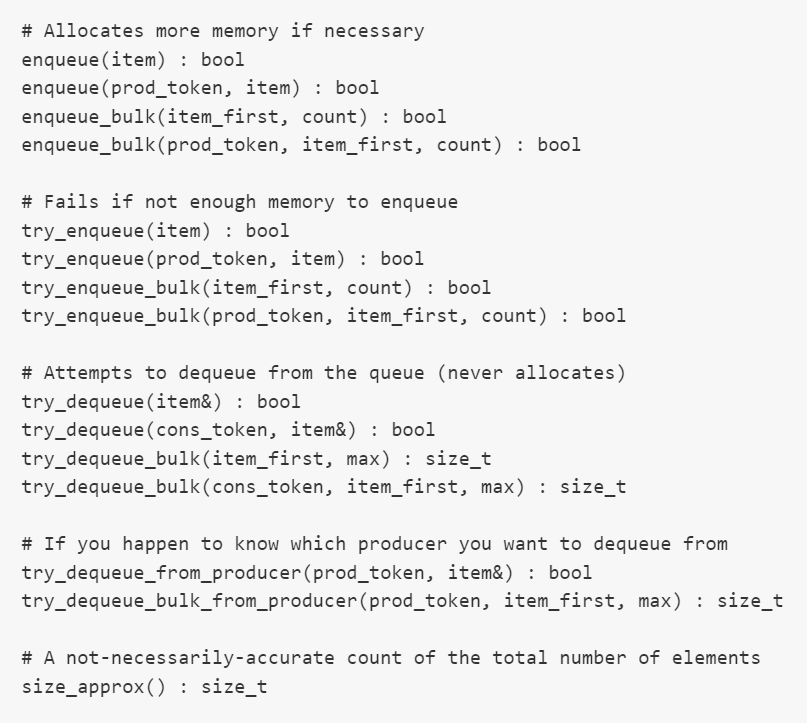
\includegraphics[width=0.8\textwidth]{moody}
        \caption{The API of the \texttt{moodycamel::concurrentqueue}}
\end{figure}

The only troublesome method is \texttt{size\_approx()} because it cannot be determined for a consuming thread if the queue is complete empty or if some enqueue operations did not propagate their memory-state to the asking thread. The proposed solution to the problem with \texttt{size\_approx()} from the developer was the use of memory barriers. How they were implemented is described in Chapter 4.
\subsection{Serial Port Wrapper}
The Serial-Port class was developed from Terraneo Federico \cite{serport}. It is a very simple wrapper around the Boost.Asio serial port components and simplifies the work with serial ports. It allows to set a timeout on the serial port to detect transmission pauses. All functionality could be done with standard Boost.Asio operations, but the code used e.g. to open a serial port consists of many lines. With this wrapper a serial port can be opened in one line, only by specifying the port name as well as the desired Baud rate.